\chapter{DUNE-PRISM}
\label{ch:prism}

%%%%%%%%%%%%%%%%%%%%%%%%%%%%%%%%
\section{Overview of DUNE-PRISM}
\label{sec:prism-ovvw}

A fundamental challenge for previous accelerator-based neutrino oscillation experiments, including T2K and NOvA, has been the precision with which neutrino-nucleus interactions can be modeled. Neutrino oscillation probabilities are a function of the neutrino energy, so any bias in the determination of the neutrino energy will produce biases in the measured neutrino oscillation parameters. The reconstructed neutrino energy in a neutrino-nucleus interaction is determined from the kinematics of the observed final state particles. Hence, if the relationship between true neutrino energy and final state particle kinematics is mismodeled, the measured oscillation parameters can deviate from their true values.

%At the GeV energy scale, where long-baseline neutrino experiments are generally conducted, several types of neutrino interactions are possible. At the lower energies (below 1~GeV), charged-current, quasi-elastic (CCQE) interactions, in which a single lepton and nucleon are in the final state, dominate the cross section. At somewhat higher energies, the target nucleon can be excited into a resonance state and produce a nucleon and a pion, along with the charged lepton, in the final state (CC1$\pi$). At even higher energies, Deep Inelastic Scattering (DIS) between a neutrino and a quark produce multi-hadron final states. In the DUNE neutrino beam, each of these processes contribute to the observed neutrino event sample.

%Further complicating ... nuclear effects: multi-nucleon, FSI, Fermi momentum, binding energy.

Neutrino-nucleus interactions at the GeV scale are difficult to model for several reasons, including the presence several different overlapping neutrino-nucleon exclusive processes, such as charged-current quasi-elastic (CCQE), charged-current resonant pion production (CCRES), and deep inelastic scattering (DIS) interactions. These neutrino-nucleon interactions take place within an argon nucleus, which results in a variety of nuclear effects, such as long- and short-range correlations with other nucleons, final state interactions of particle produced in the initial interaction, the Fermi motion of the target nucleons, and nuclear binding energy.

Neutrino energy reconstruction bias occurs when final state particle mismodeling is coupled with detector effects. When neutrons interact inelastically with argon nuclei, only a small fraction of the neutron kinetic energy is converted into detectable ionization energy (e.g. via protons). Much of the rest of the energy is lost to undetectable nuclear binding energy used to liberate nucleons from the parent argon nucleus, and to neutrons escaping the detector. This results in a feed-down of reconstructed neutrino energy relative to the true neutrino energy. Other detector effects, such as misidentifying a charged pion as a proton, can produce a large bias in the reconstructed neutrino energy.

In all previous long-baseline neutrino experiments, a near detector was used to sample neutrinos from a single unoscillated energy spectrum to constrain parameters of both the neutrino flux and neutrino-nucleus interaction models. These constrained models were used to predict the oscillated far detector reconstructed neutrino energy distribution, which was then compared to data to determine the oscillation parameter values. However, if the neutrino-nucleus model used in such a procedure is incorrect, it is possible for the near-detector-constrained model to produce an incorrect far detector event rate prediction. This effect is particularly problematic for long-baseline neutrino oscillation experiments, where the near and far detector distributions are very different for both muon and electron neutrinos. As shown in Figure~\ref{fig:nearfarenu}, the near detector energy spectra a very broad relative to the more feature-rich far detector energy spectra. A feed-down in reconstructed neutrino energy relative to the true neutrino energy can have a much larger impact on the measured far detector $\nu_\mu$ and $\nu_e$ event distributions. A detailed demonstration of the potential bias in the measured neutrino oscillation parameters due to this type of neutrino-nucleus mismodeling is given in the DUNE Conceptual Design Report~\cite{DUNECDR}.

\begin{dunefigure}[DUNE $\nu_\mu$ and $\nu_e$ Energy Spectra]{fig:nearfarenu}
{The $\nu_\mu$ (left) and $\nu_e$ (right) energy spectra are shown at both the far detector (orange), and the near detector in the on-axis position (blue).}
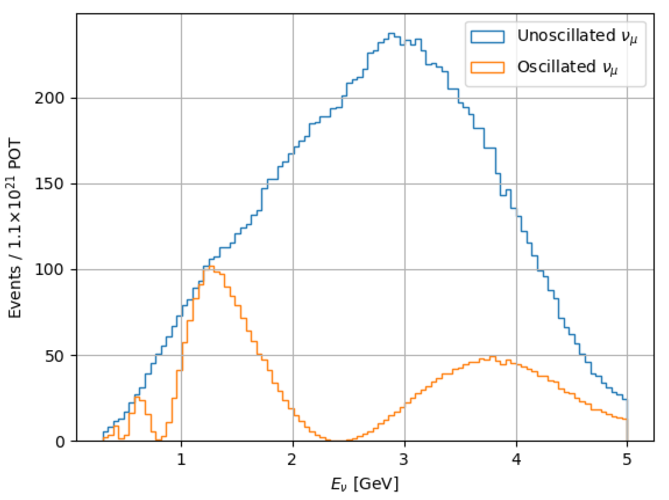
\includegraphics[width=0.45\textwidth]{graphics/prism/numuflux.pdf}
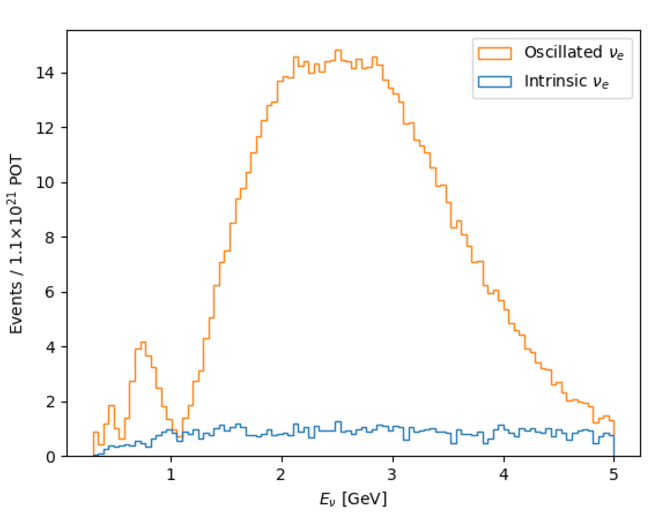
\includegraphics[width=0.45\textwidth]{graphics/prism/nueflux.pdf}
\end{dunefigure}

The DUNE-PRISM (Precision Reaction-Independent Spectrum Measurement) near detector measurement program addresses these issues by measuring neutrinos over many different neutrino energy spectra. This is achieved by moving the liquid argon near detector to a variety of positions off-axis from the neutrino beam direction. Since the beam neutrinos are produced by the decays of forward-focused charged particle parents, as the detector moves further off-axis, the peak energy of the neutrinos is reduced, and the spectrum becomes narrower. By continuously sampling these spectra over the full far detector energy range, the relationship between the true and reconstructed neutrino energy spectrum can be directly constrained.

%%%%%%%%%%%%%%%
\subsection{Introduction and Scope}
\label{sec:prism-ovvw-intro}

The DUNE-PRISM near detector system consists of components directly related to the movement of the liquid argon detector (ND-LAr) and the temporary muon spectrometer (TMS). The scope includes a set of Hilman motorized chain skates~\cite{hilmanpatent}, which will be attached to the bottom of each detector frame. The skates travel along 2-inch-think steel tracks that run the length of the near detector hall. Also within the DUNE-PRISM scope are a set of ``\dwords{echain}'' that contain all of the utilities (cryogenic lines, power, data cables, etc.) that run to each detector. Finally, motion monitoring systems, including a laser positioning system, accelerometers, and vibration monitors, are within the DUNE-PRISM scope.

%%%%%%%%%%%%%%% Not in Tim's new organization
\subsection{Principle of Operation}
\label{sec:prism-ovvw-op}

Each Hilman skate is powered by servo motors that controlled by a manufacturer-supplied control unit. The control system allows for custom control of the detector speed, acceleration, and jerk. A built-in encoder is used to determine the instantaneous position within the cavern and initiate motion changes to reach any specified target location. Each of the 2 mobile detectors will have an independent skate + control system, which will move in unison during normal operating conditions.

%%%%%%%%%%%%%%%
\subsection{Design Parameters}
\label{sec:prism-ovvw-param}

The design parameters are specified in the DUNE-PRISM section of the detector capabilities listed in Table~\ref{tab:spec:nd-cap}. The detector design allows for a maximum off-axis travel distance of 28.5~m to cover the far detector oscillation energy range. The beam flux and detector performance can vary on a distance scale of 10~cm, so a detector placement precision of 3~cm is required to allow for matching of high-efficiency regions within the detector with any particular off-axis location at the $3~\sigma$ level. Once the detector movement has ceased, the achieved detector location must be measured with a precision requirement of 1~cm, and a precision goal 1~mm, to ensure the knowledge of the detector location has an uncertainty equal to or smaller than the alignment precision of components within each detector.

To ensure a full suite of off-axis measurements is achieved with minimal variations in beam and detector conditions, the system is designed to allow for weekly detector position changes between any 2 detector positions within the hall. To keep near detector downtime due to detector movement to <5\%, each movement must be completed within an 8 hour time window. This includes 1 hour of preparation time prior to movement, up to 6 hours of detector motion, and 1 hour following the movement to restore detectors to data-taking condition. This requires a detector top-speed of at least 10~cm/min, and an acceleration of at least 0.17 cm/min$^2$.
%\dword{duneprism} is designed to meet the physics requirements of the \dword{dune} experiment. 
%A summary of the design parameters are given in Table~\ref{tab:table-prism-params}. 


%\begin{dunetable}
%[Placeholder for parameter table]
%{cc}
%{tab:table-prism-params}
%{Placeholder for Parameter Table - it will be generated from a spreadsheet}
%Rows & Counts \\ \toprowrule
%Row 1 & First \\ \colhline
%Row 2 & Second \\ \colhline
%Row 3 & Third \\ % no \colhline on final row
%\end{dunetable}

%%%%%%%%%%%%%%% Not in Tim's new organization
\subsection{Performance}
\label{sec:prism-ovvw-perf}

The DUNE-PRISM system must be able to move both the fully instrumented and liquid-argon-filled ND-LAr detector, and the TMS detector, with minimal disruption to detector hardware components and services. Targeted studies have been performed to understand the motion of the liquid argon due to accelerations and vibrations. 

A hydrodynamics simulation analysis was performed to determine the impact of accelerating the filled ND-LAr cryostat. The maximum height of waves formed during the motion was found to be linear with detector acceleration. At the minimum acceleration required for motion, 0.17 cm/min$^2$, wave formation is negligible. At the maximum acceleration of the Hilman skates, 0.25 cm/s$^2$ ($\sim 5000 x$ larger), a maximum wave height of 3~mm is expected, which is small relative to the 39.6~cm ullage height above the liquid phase. The damping period is 7.5~minutes, so any waves formed during the acceleration phase will dissipate during the constant velocity phase, prior to deceleration. Wave formation due to vibration is expected to be heavily damped, and not contribute significantly to wave formation. During the acceleration phase, the outer-most ArgonCube module G10 wall within ND-LAr experiences the highest pressure. However, at 0.25 cm/s$^2$, this results in a deformation of only 0.17~mm at the center of the wall. Overall, fluid motion is not expected to produce any negative impact on the ND-LAr detector for any of the motion parameters achievable by the Hilman skates.

In order to take data over the full off-axis range within a nominal DUNE beam run (which assumes a 56\% uptime), the movement system is designed to move at least once per week. In particular, the cryogenics flexible, particularly the vacuum jacketed liquid argon and liquid nitrogen supply lines that will be housed inside the DUNE-PRISM ND-LAr \dword{echain}, have been chosen to withstand up to 1000 coiling / uncoiling cycles to account for this movement.
A sample run plan is shown in Table~\ref{tab:runplantable}, in which roughly half the time is spent on-axis. This can provide sufficient statistics at the far off-axis locations while provide a large dataset on-axis to constrain the neutrino flux via interactions such as $\nu-e^-$ scattering.

\begin{dunetable}
[Example 1 year PRISM run plan and event rates]
{|c|c|c|c|c|c|c|}
{tab:runplantable}
{A sample run plan is outlined, for which approximately half of the assumed 29 week beam-year the detector is in the  on-axis position, one week is spent on axis but with a lower horn current (280 kA), and the remaining time is evenly divided between off-axis positions. The fiducial volume assumed is 4\,m wide, with the largest off axis position sampled at 32.5\,m, The table shows the rate of $\nu_\mu$ CC events before ($N_{\nu_\mu CC}$) and after (N$_{Sel}$) the \dword{nd} event selection, the fraction of wrong-sign background (WSB), the fraction of neutral current events (NC). The total number of $\nu_\mu$ CC interactions in the gas is also provided.} 
% \multicolumn{2}{|c|}{} & \multicolumn{4}{|c|}{Liquid} & Gas\\ \hline
 \span\omit  & \multicolumn{4}{|c|}{ND-LAr} & ND-GAr\\ \hline
 \multicolumn{2}{|c|}{} & All int. &\multicolumn{3}{|c|}{Selected} & All int. \\
\hline
Stop&Run duration&N$_{\nu_{\mu}CC}$ & N$_{Sel}$ & WSB & NC & N$_{\nu_{\mu}CC}$ \\
\hline
On axis (293 kA)\,m & 14 wks. & 21.6M & 10.1M & 0.2\% & 1.3\% & 580,000\\
On axis (280 kA)\,m & 1 wk. & 1.5M & 690,000 & 0.3\% & 1.3\% & 40,000\\
4 m off axis\,m & 12 dys. & 2.3M & 1.2M & 0.3\% & 1.0\% & 61,000\\
8 m off axis\,m & 12 dys. & 1.3M & 670,000 & 0.5\% & 0.9\% & 35,000\\
12 m off axis\,m & 12 dys. & 650,000 & 330,000 & 0.8\% & 0.7\% & 17,000\\
16 m off axis\,m & 12 dys. & 370,000 & 190,000 & 1.1\% & 0.7\% & 10,000\\
20 m off axis\,m & 12 dys. & 230,000 & 120,000 & 1.3\% & 0.7\% & 6,200\\
24 m off axis\,m & 12 dys. & 150,000 & 75,000 & 1.8\% & 0.7\% & 4,100\\
28 m off axis\,m & 12 dys. & 110,000 & 50,000 & 2.1\% & 0.8\% & 2,900\\
30.5 m off axis\,m & 12 dys. & 87,000 & 39,000 & 2.3\% & 0.7\% & 2,300\\
\end{dunetable}


%%%%%%%%%%%%%%%%%%%%%%%%%%%%%%%%
\section{System Design}
\label{sec:prism-des}

The DUNE-PRISM system is designed to move 2 individual detectors along a straight path up to 30.5m in length.  The system consists of a group of powered skates which can provide high-precision controlled movement, and a set of \dwords{echain} to carry power, data, and utilities to and from each detector at any arbitrary position along the detector travel path.  Each detector will require one set of skates and 2 energy chains: one for power a data cables, and one for utilities such as cryogenic fluids and an air supply line.

%%%%%%%%%%%%%%%
\subsection{Moving a Loaded Cryostat}
\label{sec:prism-des-move}

The DUNE-PRISM system is unlike any previous system for moving large detector components, as the detectors will be moved on a regular basis (weekly) with minimal preparation time prior to a movement, and minimal recovery time following a movement before data taking is restarted. This places more stringent requirements on the precision of motion control required, the degree to which the movements must be automated, and the smoothness with which the motion takes place. 

%%%%%%%%%%%%%%% One subsection for each WBS element:
\subsection{Movement System}
\label{sec:prism-des-wbs1}
\begin{itemize}
    \item Hilman skates
    \item Rails~\ref{fig:prismrails} and cavern connection hardware
    \item Control box and interface to DUNE-ND slow controls
\end{itemize}

\begin{dunefigure}[DUNE-PRISM Rail System]{fig:prismrails}
{The DUNE-PRISM rail system within the near detector cavern is shown. The 4 primary rails for the TMS and ND-LAr run the length of the hall, and 2 sets of cross rails allow the SAND detector to cross between sets of primary rails and enter the SAND alcove.}
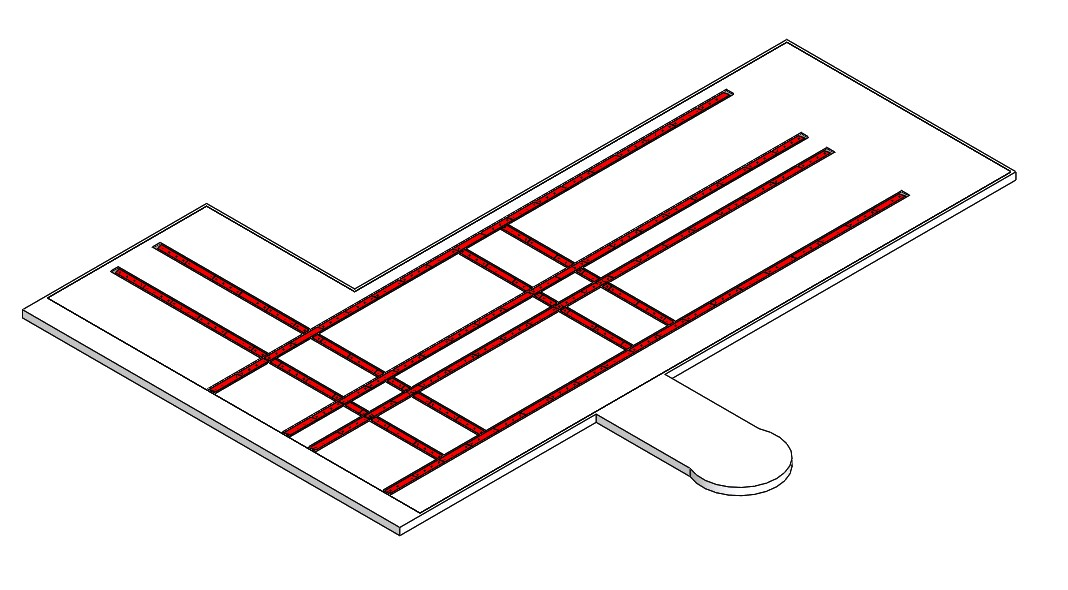
\includegraphics[width=0.98\textwidth]{graphics/prism/prismrails.jpg}
\end{dunefigure}

%%%%%%%%%%%%%%% One subsection for each WBS element:
\subsection{Energy Chains}
\label{sec:prism-des-wbs2}
\begin{itemize}
    \item ND-LAr utilities energy chain (flexible cryogenics lines)
    \item ND-LAr power and data energy chain
    \item TMS utilities energy chain
    \item TMS power and data energy chain
\end{itemize}

%%%%%%%%%%%%%%% One subsection for each WBS element:
\subsection{Monitoring and Safety Systems}
\label{sec:prism-des-wbs3}
\begin{itemize}
    \item Built in position encoder on Hilman skates
    \item Laser positioning system
    \item Accelerometers / vibration monitors
    \item Safety systems
\end{itemize}


% %%%%%%%%%%%%%%% Maybe not needed?
% \subsection{Infrastructure and Tooling}
% \label{sec:prism-des-infr}

% %%%%%%%%%%%%%%% Maybe falls under WBS elements?
% \subsection{Auxiliary Pieces and Instrumentation}
% \label{sec:prism-des-aux}

%%%%%%%%%%%%%%%%%%%%%%%%%%%%%%%%
\section{Interfaces}
\label{sec:prism-interface}

Table~\ref{tbl:larndinterfaces} contains a summary and brief description of all the interfaces between the \dword{duneprism} system and other consortia, working groups, and task forces.
%, with references to the current version of the interface documents describing those interfaces.  
Drawings of the mechanical interfaces and diagrams of the electrical interfaces are 
included in the interface documents as appropriate.
It is expected that further refinements of the interface documents will take place prior to the final \dword{prr} for the detector. The interface documents specify the responsibility of different consortia or groups during all phases of the experiment including design and prototyping, integration,  installation, and  commissioning.


\begin{dunetable}
[\dshort{duneprism} interface links]
{p{0.25\textwidth}p{0.5\textwidth}l}
{tbl:larndinterfaces}
{\dshort{duneprism} interface links}
Interfacing System & Description & Linked Reference \\ \toprowrule
Attachment of rails to the cavern floor     &  Near Detector Conventional Facilities, in coordination with ND I\&I, will provide anchors to attach the rails to the cavern floor.
& \citedocdb{?} \\ \colhline

Energy chains, Connection to cavern walls &  Near Detector Conventional Facilities, in coordination with ND I\&I, will provide wall anchors to which the DUNE-PRISM energy chain support structure will be attached.
& \citedocdb{?} \\ \colhline

Energy chains, Connection to detectors & The energy chains will be attached to access points provided by the TMS and the ND-LAr cryostat groups (e.g. see Figure~\ref{fig:chainndlar}).
& \citedocdb{?} \\ \colhline

Energy chains, Detector services to be run through the chains  &  The cryogenics group will provide the flexible hoses that run through the large ND-LAr energy chain. Power and data cables will be provided by I\&I, and will terminate in racks on the TMS and ND-LAr cryostat.
& \citedocdb{?} \\ \colhline

Connection from Hilman skates to detector platforms &  The platforms for TMS and ND-LAr will provide attachment points for the Hilman skates.
& \citedocdb{?} \\

Power and data for Hilman skates and control system &  The platforms for TMS and ND-LAr will provide power to the skates, and power and data cables to the Hilman control box.
& \citedocdb{?} \\
\end{dunetable}

\begin{dunefigure}[DUNE-PRISM Energy Chain Interface to ND-LAr]{fig:chainndlar}
{The connection of the energy chain to the ND-LAr detector is shown.}
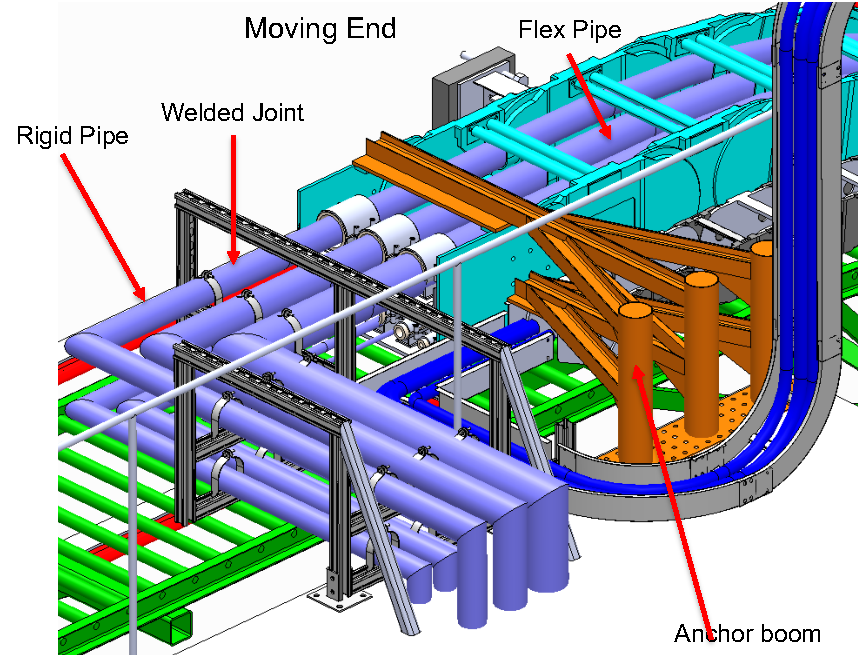
\includegraphics[width=0.8\textwidth]{graphics/prism/ndlar_energychain.pdf}
\end{dunefigure}


%%%%%%%%%%%%%%%%%%%%%%%%%%%%%%%%
\section{Risks and Mitigations}
\label{sec:prism-risks}

%Table~\ref{tab:table-prism-risks} 
Figure~\ref{fig:prismrisks} contains a list of all the
risks that \dword{dune} is currently holding in the \dword{duneprism} risk register.  Each line includes the official \dword{dune} risk register identification number, a description of the risk, the proposed mitigation for the risk, and finally three columns rating the post-mitigation (P)robability that the risk described comes to pass, the degree of (C)ost risk for that line, and the degree of (S)chedule risk.  Risk levels are defined as (L)ow (<10\% probability of occurring, <5\% cost impact, <2 month schedule impact), (M)edium (10 to 25\% probability of occurring, 5\% to 20\% cost impact, 2 to 6 month schedule impact), or (H)igh (>25\% probability of occurring, >20\% cost impact, >6 month schedule impact).  Most of these risks are reduced to a ``Low'' level following mitigation (as shown in the table), although several of them currently hold a higher risk levels (pre-mitigation), due to the early stage of development of the \dword{duneprism} system relative to other systems.  

%A narrative description of each of the risks and the proposed mitigation is given in the risk table shown in Figure~\ref{fig:prismrisks}.

\fixme{Anne needs to get risk table template put together; below from google sheet}

\begin{dunefigure}[DUNE-PRISM Risk Table]{fig:prismrisks}
{The proposed risks for DUNE-PRISM are given in the table.}
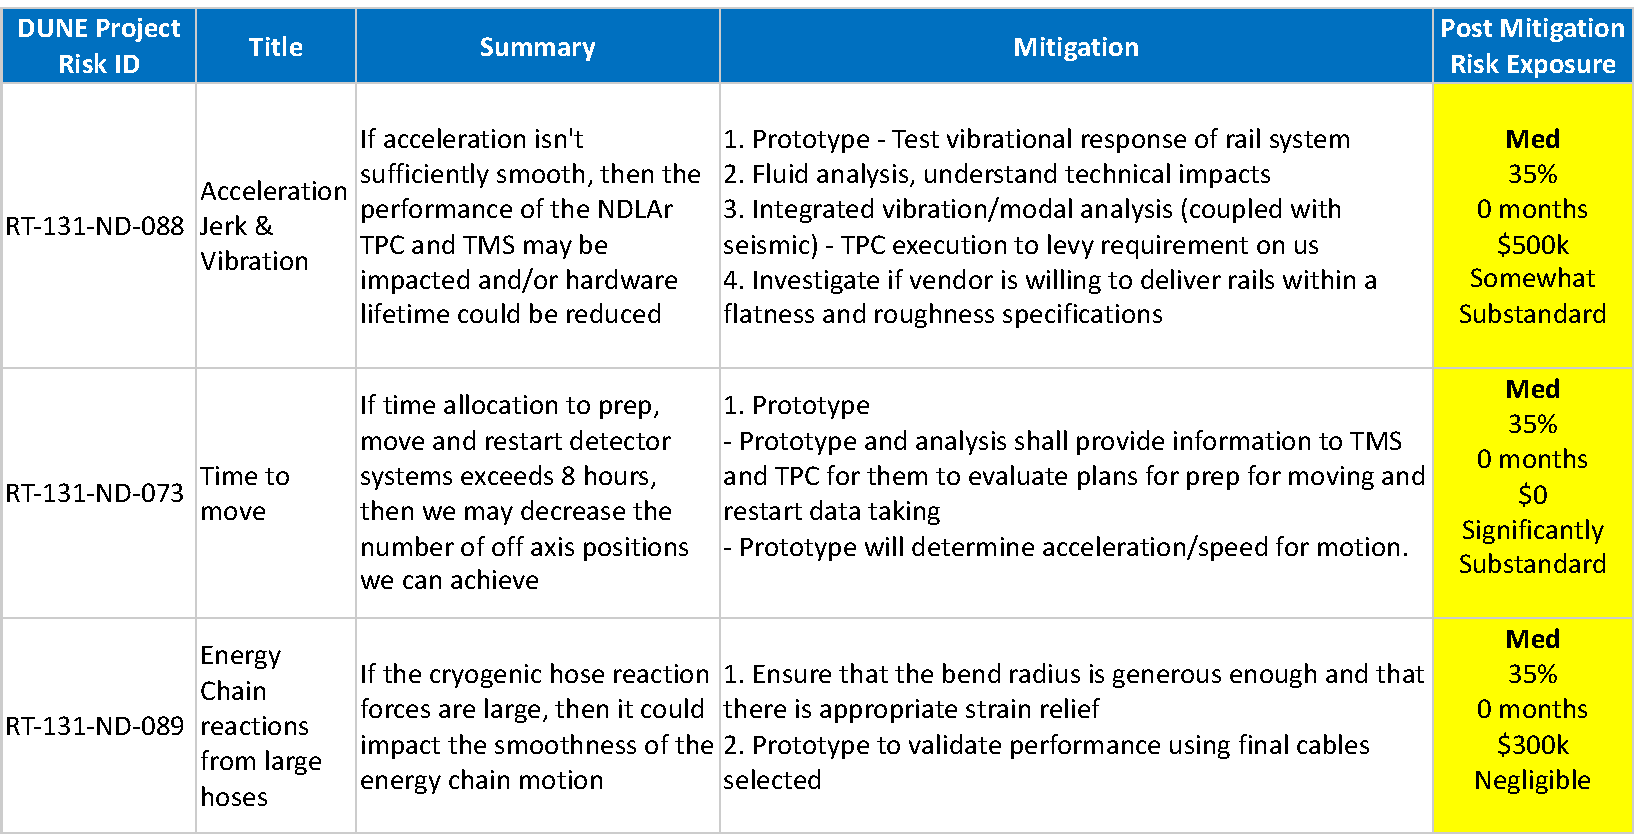
\includegraphics[width=0.98\textwidth]{graphics/prism/prismrisks.pdf}
\end{dunefigure}


%\input{generated/risks-longtable-ND-LAr.tex}

%\begin{dunetable}
%[Placeholder for risks table]
%{cc}
%{tab:table-prism-risks}
%{Placeholder for Risks Table - it will be generated from a %spreadsheet}
%Rows & Counts \\ \toprowrule
%Row 1 & First \\ \colhline
%Row 2 & Second \\ \colhline
%Row 3 & Third \\ % no \colhline on final row
%\end{dunetable}

%%%%%%%%%%%%%%%%%%%%%%%%%%%%%%%%
\section{Schedule}
\label{sec:prism-org-sched}

%Table \ref{tab:prism-sched}
Figure~\ref{fig:prismsched} lists key milestones in the design, validation, construction, and installation of both the prototype and the full \dword{duneprism} system.

% \fixme{Anne to get list of main DUNE sched items from Eric J before making the real table template}
% \begin{longtable}
% {p{0.75\textwidth}p{0.25\textwidth}}
% \caption{\dshort{duneprism} system consortium schedule}\\ \colhline
% \rowcolor{dunetablecolor}Milestone & Date   \\ \toprowrule


% \rowcolor{dunepeach}Beneficial occupancy of cavern 1 and \dword{cuc}& \cucbenocc      \\ \colhline
% Initial batch (80 PD modules) assembled  & March 2023\\ \colhline

% \rowcolor{dunepeach}Top of \dword{detmodule} \#1 cryostat accessible& \accesstopfirstcryo      \\ \colhline
% Third batch (320 PD modules) arrive at US PD Reception Facility  & January 2024\\ 

% \label{tab:prism-sched}
%\end{longtable}

\begin{dunefigure}[DUNE-PRISM Risk Table]{fig:prismsched}
{The DUNE-PRISM key milestones and activities are shown.}
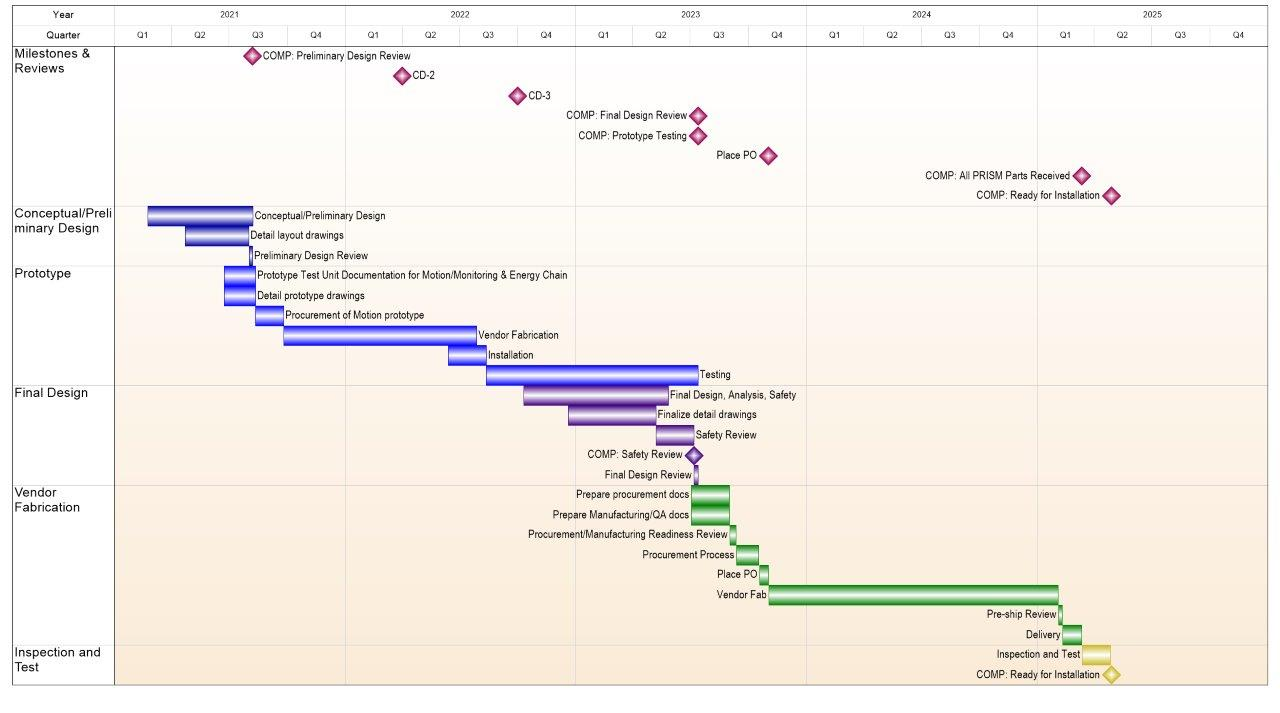
\includegraphics[width=0.98\textwidth]{graphics/prism/PRISM2020DecR2.jpg}
\end{dunefigure}


%%%%%%%%%%%%%%%%%%%%%%%%%%%%%%%%
\section{Prototyping Plans}
\label{sec:prism-qc}

The primary components of the DUNE-PRISM system, the power Hilman skate movement system and the energy chains, are commercial products that have been implemented in a variety of industrial applications. For this reason, no proof-of-concept prototype is required prior to CD-2. However, there are risks associated with the precision with which the system can be controlled, the impact of vibrations on the performance and longevity of detector hardware, and the performance of the rolling/unrolling of the energy chain. To understand these risks, and to develop the movement control integration and interfaces to the detector monitoring systems, an engineering-test-unit prototype will be designed and operated prior to the final system design.


The Hilman motion control system, and monitoring systems, must be integrated into the DUNE slow-controls framework. Starting and stopping procedures must be defined, including acceleration and jerk (acceleration rate-of-change) parameters. Other special controls scenarios, including emergency stop procedures, will be defined and tested. The laser positioning system and acceleration/vibration monitors will also be integrated and tested.

The prototype consists of a steel platform that rests upon 4 powered Hilman skates. The skates move along a set of 2 rails, each 61'4" in length, which will allow the prototype to test the accelerations and velocities planned for the final detector. On top of the platform is a rectangular water tank surrounded by concrete shielding blocks, which are currently present in the lab. An energy chain containing vacuum-jacketed cryogenic hoses will be attached to the detector and run alongside the rails.

The prototype will be built in a large basement lab at Stony Brook University. The lab is 130' long along the direction of travel, and 33' wide, which is sufficient to test rail spacings and travel distances similar to those used for the ND-LAr detector. There is a 7.5 ton crane that runs the length of the lab, and sufficient electricity and water supply to fill an operate the system.


\begin{dunefigure}[DUNE-PRISM Prototype]{fig:prismprototype}
{The left figures show the prototype design with 4 power Hilman skates, a steel platform, and a large mass of concrete blocks and water. The right figure shows a schematic of the prototype laboratory at Stony Brook University.}
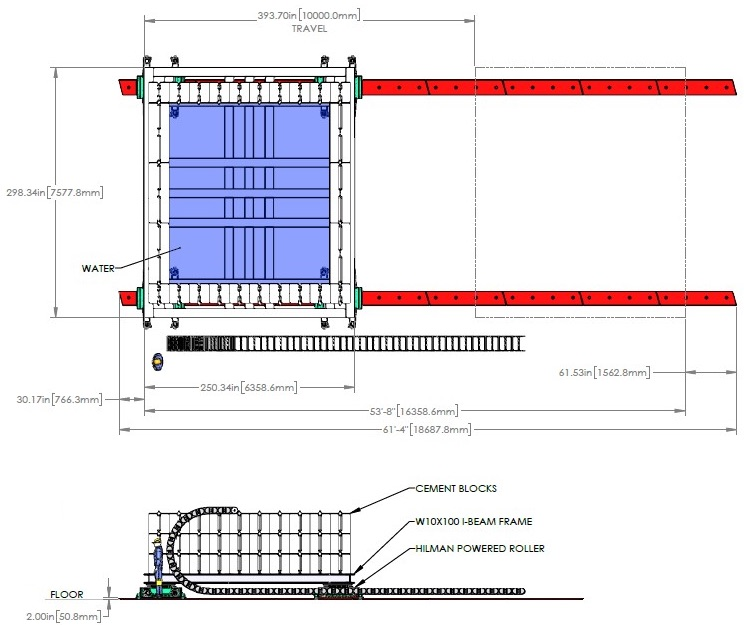
\includegraphics[width=0.75\textwidth]{graphics/prism/prismprototype.jpg}
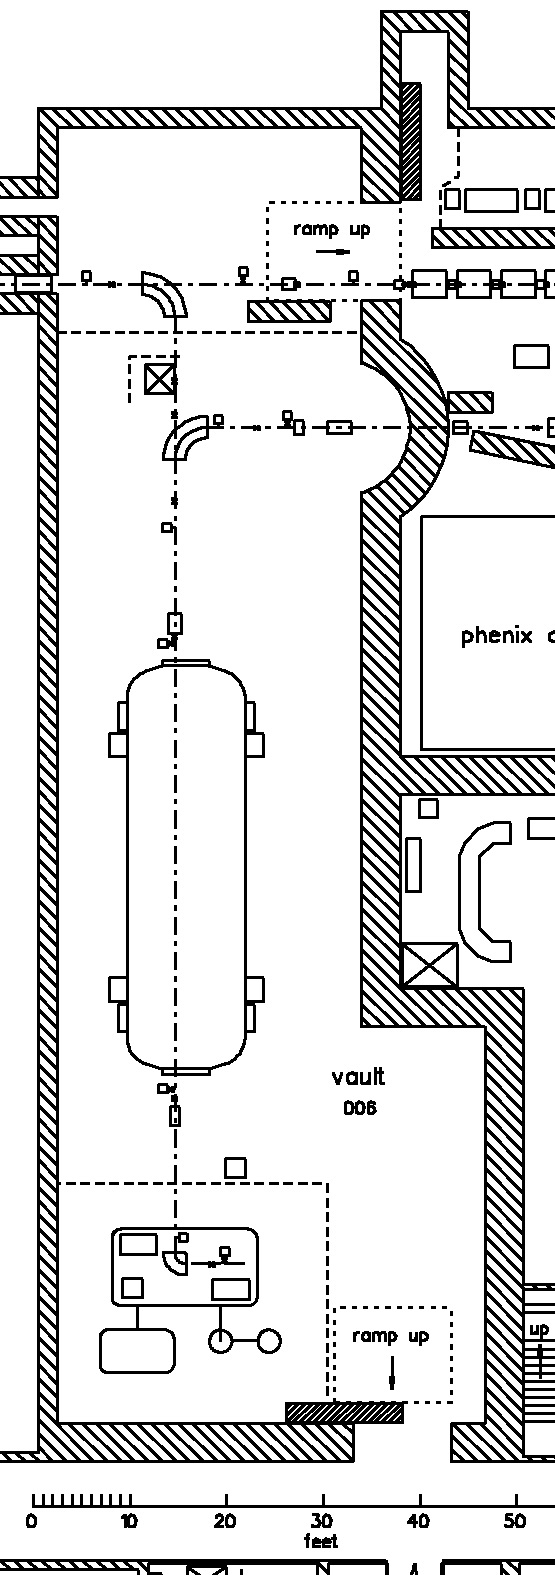
\includegraphics[width=0.23\textwidth]{graphics/prism/sbulab.jpg}

\end{dunefigure}


\begin{comment}. %%%%% comment here to end
\fixme{The following sections are not in the new structure; I'm keeping them at the end here for now, in case you want to include one or more of them later.}

%%%%%%%%%%%%%%%%%%%%%%%%%%%%%%%% Not in Tim's new organization
\section{Safety Concerns}
\label{sec:prism-safety}

%%%%%%%%%%%%%%%%%%%%%%%%%%%%%%%%
\section{Calibration}
\label{sec:prism-calib}

%%%%%%%%%%%%%%%%%%%%%%%%%%%%%%%%
\section{Quality Assurance}
\label{sec:prism-qa}

%%%%%%%%%%%%%%%%%%%%%%%%%%%%%%%%
\section{Production, Assembly, and Quality Control}
\label{sec:prism-qc}

%%%%%%%%%%%%%%%%%%%%%%%%%%%%%%%%
\section{Transport and Handling}
\label{sec:prism-transport}

%%%%%%%%%%%%%%%%%%%%%%%%%%%%%%%%
\section{Installation, Integration, and Commissioning}
\label{sec:prism-iic}

%%%%%%%%%%%%%%%%%%%%%%%%%%%%%%%%
\section{Organization}
\label{sec:prism-org}

%%%%%%%%%%%%%%%
\subsection{Participating Institutions}
\label{sec:fdsp-org-inst}
%\metainfo{\color{red}\bf  Content: Segreto/Warner}

The \dword{duneprism} consortium benefits from the contributions of many institutions and facilities in \fixme{several countries? or the U.S. and ??}.  Table~\ref{tab:prism-institutes}
lists the member institutions. 

\begin{longtable}
{ll}
\caption{\dshort{duneprism} consortium institutions}\\ \colhline
\rowcolor{dunetablecolor} Member Institute  &  Country       \\  \toprowrule
univ 1 &  \\ \colhline
univ 2 &  \\ \colhline
univ 3 &  \\ 
\label{tab:prism-institutes}
\end{longtable}

\end{comment}









